% !Mode:: "TeX:UTF-8"

\begin{frame}{第二十讲、重积分的应用}
	\linespread{1.5}
	\begin{enumerate}
	  \item {\bf 内容与要求}{\b (\S 11.4)}
	  \begin{itemize}
		\item 质量
		\item 质心
		\item 转动惯量
	    \item 物体对质点的引力
	    \item 空间曲面的表面积*
	  \vspace{1em}
	  \end{itemize}
	  \item {\bf  课后作业:}
	  \begin{itemize}
	    \item {\b 习题11.4:1,4,6(2),9,12}
	  \end{itemize}
	\end{enumerate}
\end{frame}

\section{质量}

\begin{frame}{质量}
	\linespread{1.2}
	\begin{exampleblock}{{\bf 例1}\hfill}
		设一平面三角形薄片以$O(0,0),A(1,0),B(0,1)$为顶点,
		其上任一点$(x,y)$处的面密度$\mu(x,y)=x^2+y^2$,
		求该平面薄片的质量。
	\end{exampleblock}
	\pause
	{\bb 平面物体的质量}
	$$\alert{m=\iint_D\mu(x,y)\d\sigma}$$
	\pause
	{\bb 三维空间立体体积}
	$$\alert{m=\iiint_{\Omega}\mu(x,y,z)\d V}$$
\end{frame}

\section{质心}

\begin{frame}{质心(重心、形心)}
	\linespread{1.2}\pause 
	{\bb 空间$n$个质点的质心:}\pause
	
	空间中$n$个质点($k=1,2,\ldots,n$),质量分别为$m_k$,坐标$(x_k,y_k,z_k)$\pause
	$$\alert{\bar{x}=\df{\sum\limits_{k=1}^nx_km_k}{\sum\limits_{k=1}^nm_k},}\;\pause
	\alert{\bar{y}=\df{\sum\limits_{k=1}^ny_km_k}{\sum\limits_{k=1}^nm_k},}\;\pause 
	\alert{\bar{z}=\df{\sum\limits_{k=1}^nz_km_k}{\sum\limits_{k=1}^nm_k}}$$
\end{frame}

\begin{frame}{质心}
	\linespread{1.2}
	{\bb 平面薄片的质心:}\pause 密度函数$\mu(x,y)$,$(x,y)\in D$\pause
	$$\alert{\bar{x}=\df{\displaystyle\iint_Dx\mu(x,y)\d\sigma}
	{\displaystyle\iint_D\mu(x,y)\d\sigma},\;}\pause 
	\alert{\bar{y}=\df{\displaystyle\iint_Dy\mu(x,y)\d\sigma}
	{\displaystyle\iint_D\mu(x,y)\d\sigma}}$$
	\pause
	\begin{exampleblock}{{\bf 例2}\hfill}
		设半径为$R$的半圆形薄片上每一点的面密度与该点到圆心的距离成正比,
		求该薄片的质心。
	\end{exampleblock}
\end{frame}

\begin{frame}{质心}
	\linespread{1.2}\pause 
	{\bb 空间物体的质心:}\pause 密度函数$\mu(x,y,z)$,$(x,y,z)\in\Omega$\pause
	$$\alert{\bar{x}=\df{\displaystyle\iiint_{\Omega}x\mu(x,y,z)\d V}
	{\displaystyle\iiint_{\Omega}\mu(x,y,z)\d V},\;}\pause
	\alert{\bar{y}=\ldots,\;\bar{z}=\ldots}\pause
% 	\alert{\bar{y}=\df{\displaystyle\iiint_{\Omega}y\mu(x,y,z)dV}
% 	{\displaystyle\iiint_{\Omega}\mu(x,y,z)dV},\;}\pause $$
% 	$$\alert{\bar{z}=\df{\displaystyle\iiint_{\Omega}z\mu(x,y,z)dV}
% 	{\displaystyle\iiint_{\Omega}\mu(x,y,z)dV}}
	$$
	\begin{exampleblock}{{\bf 例3}\hfill}
		求均匀半球壳
		$\Omega:a^2\leq x^2+y^2+z^2\leq b^2$
		的形心。
	\end{exampleblock}
\end{frame}

% \begin{frame}
% 	\linespread{1.2}
% 	\begin{exampleblock}{{\bf 例3}\hfill}
% 		求均匀半球壳
% 		$\Omega:a^2\leq x^2+y^2+z^2\leq b^2$
% 		的形心。
% 	\end{exampleblock}
% 	\begin{center}
% 		\pause \resizebox{!}{5cm}{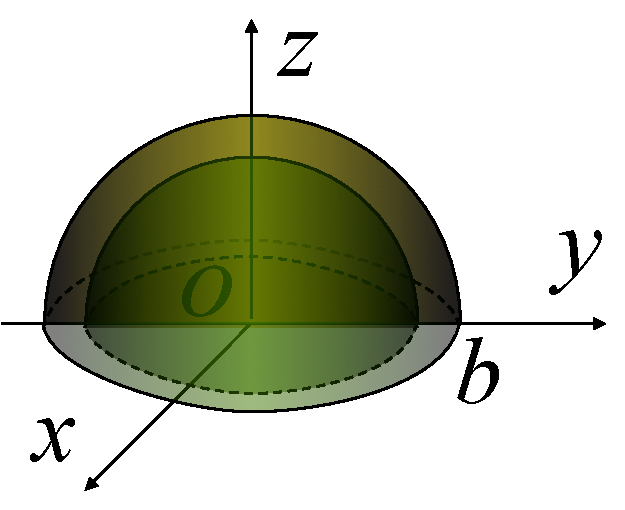
\includegraphics{./images/ch11/2s.pdf}}
% 	\end{center}
% \end{frame}

\section{转动惯量}

\begin{frame}{转动惯量}
	\linespread{1.2}\pause 
	\begin{columns}
		\column{.5\textwidth}
		{\bb 空间一质点的转动惯量:}
			$$\alert{I=mr^2}$$
		\column{.5\textwidth}
			\begin{center}
				\pause \resizebox{!}{4cm}{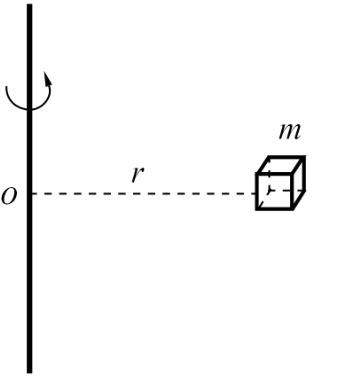
\includegraphics{./images/ch11/roll.pdf}}
			\end{center}
	\end{columns}
	{\bb \pause 空间物体绕$z$轴旋转:}\pause 密度函数$\mu(x,y,z),(x,y,z)\in\Omega$\pause
	$$\alert{I=\iiint_{\Omega}(x^2+y^2)\mu(x,y,z)\d V}$$
\end{frame}

\begin{frame}
	\linespread{1.2}
	\begin{exampleblock}{{\bf 例5}\hfill}
		求半径为$R$的均匀半圆形薄片绕其平分线转动的转动惯量和旋转半径。
	\end{exampleblock}
	\bigskip\pause 
	{\bb 转动半径:}
	$$\alert{r=\sqrt{\df{I}{m}}}$$
\end{frame}

\begin{frame}
	\linespread{1.2}
	\begin{exampleblock}{{\bf 例6}(平行轴定理)\hfill}
		设$L_c$为通过物体$\Omega$质心的直线,直线$L_t$平行于$L_c$,
		两者距离为$d$。试证:$\Omega$关于轴$L_t$的转动惯量$I_t$与物体关于轴
		$L_c$的转动惯量$I_c$之间存在关系如下:
		$$I_t=I_c+Md\,^2,$$
		其中$M$为$\Omega$的质量。
	\end{exampleblock}
\end{frame}

\section{万有引力}

\begin{frame}{万有引力}
	\linespread{1.2}
	物体$\Omega$的点密度为$\mu(x,y,z)$,质量为$m$的质点位于
	$(a,b,c)$,$\Omega$对$m$的引力为:\pause
	$$\alert{F_x=\iiint_{\Omega}Km\mu\df{x-a}{r^3}\d V,}\pause $$
	$$\alert{F_y=\iiint_{\Omega}Km\mu\df{y-b}{r^3}\d V,}\pause $$
	$$\alert{F_z=\iiint_{\Omega}Km\mu\df{z-c}{r^3}\d V} $$
\end{frame}

\begin{frame}
	\linespread{1.2}
	\begin{exampleblock}{{\bf 例7}\hfill}
		求高为$H$,底半径为$R$且密度均匀的圆柱体,对其底面中心
		一单位质量质点的引力。
	\end{exampleblock}\pause
	\begin{center}
		\resizebox{!}{5cm}{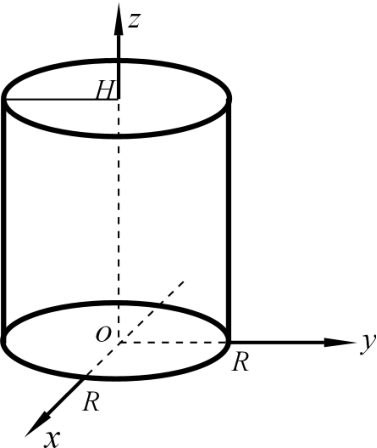
\includegraphics{./images/ch11/cg.pdf}}
	\end{center}
\end{frame}

\section{空间曲面的表面积}

\begin{frame}{空间曲面的表面积}
	\linespread{1.2}\pause
	\begin{exampleblock}{{\bf 例8}\hfill}
		已知函数$z=f(x,y)\,(x,y)\in D$,求其对应曲面的表面积。
	\end{exampleblock}
	\pause
	$$\alert{S=\iint_D\sqrt{1+(f\,'_x)^2+(f\,'_y)^2}\d\sigma}$$
	\pause
	\begin{exampleblock}{{\bf 例9}\hfill}
		求半径为$a$的球的表面积。
	\end{exampleblock}
\end{frame}

%=====================================

% \begin{frame}{title}
% 	\linespread{1.2}
% 	\begin{exampleblock}{{\bf title}\hfill}
% 		123
% 	\end{exampleblock}
% \end{frame}
% 
% \begin{frame}{title}
% 	\linespread{1.2}
% 	\begin{block}{{\bf title}\hfill}
% 		123
% 	\end{block}
% \end{frame}